\chapter{Ergebnisse}
\section{Ergebnisse bei Messung nach Aufgabenbedingungen}
\begin{table}[h!]
\begin{tabular}{c|cccc}
    Name & 50\% & 90\% & 95\% & 100\% \\
    \hline
    Quadratic Mul & 0,42 & 1,73 & 2,35 & 8,8 \\
    Quadratic Mod & 0,44 & 1,72 & 2,32 & 10,38 \\
    Quadratic XOR & 0,43 & 1,71 & 2,36 & 9,54 \\
    \hline
    Linear Mul & 0,43 & 1,87 & 2,60 & 8,93 \\
    Linear Mod & 0,42 & 1,87 & 2,64 & 10,51 \\
    Linear XOR & 0,44 & 1,91 & 2,59 & 9,83 \\
    \hline
    Triangular Mul & 0,42 & 1,71 & 2,36 & 8,85 \\
    Triangular Mod & 0,43 & 1,74 & 2,37 & 8,12 \\
    Triangular XOR & 0,43 & 1,69 & 2,35 & 9,71 \\
    \hline
    Direct Mul & 0,25 & 0,44 & 0,47 & 0,50 \\
    Direct Mod & 0,26 & 0,45 & 0,48 & 0,50 \\
    Direct XOR & 0,25 & 0,45 & 0,48 & 0,51 \\
    \hline
    Separate Mul & 0,24 & 0,44 & 0,48 & 0,50 \\
    Separate Mod & 0,25 & 0,45 & 0,47 & 0,50 \\
    Separate XOR & 0,25 & 0,46 & 0,48 & 0,51 \\
    \hline
    Coalesced Mul & 1,17 & 1,66 & 1,74 & 1,80 \\
    Coalesced Mod & 1,16 & 1,66 & 1,72 & 1,79 \\
    Coalesced XOR & 1,17 & 1,65 & 1,72 & 1,79 \\
\end{tabular}
\centering
\caption{Durchschnittliche Kollisionen bei Zugriff mit Erfolg}
\end{table}
\begin{table}[h!]
\begin{tabular}{c|cccc}
    Name & 50\% & 90\% & 95\% & 100\% \\
    \hline
    Quadratic Mul & 1,14 & 9,50 & 19,51 & - \\
    Quadratic Mod & 1,14 & 9,60 & 19,73 & - \\
    Quadratic XOR & 1,13 & 9,62 & 19,73 & - \\
    \hline
    Linear Mul & 1,16 & 11,14 & 22,45 & - \\
    Linear Mod & 1,16 & 11,01 & 23,09 & - \\
    Linear XOR & 1,17 & 11,14 & 24,24 & - \\
    \hline
    Triangular Mul & 1,12 & 9,72 & 19,94 & - \\
    Triangular Mod & 1,13 & 9,69 & 19,68 & - \\
    Triangular XOR & 1,13 & 9,74 & 19,58 & - \\
    \hline
    Direct Mul & 0,50 & 0,90 & 0,95 & 0,99 \\
    Direct Mod & 0,50 & 0,91 & 0,94 & 1,00 \\
    Direct XOR & 0,50 & 0,90 & 0,95 & 0,99 \\
    \hline
    Separate Mul & 0,50 & 0,90 & 0,95 & 0,99 \\
    Separate Mod & 0,50 & 0,90 & 0,96 & 1,00 \\
    Separate XOR & 0,50 & 0,90 & 0,95 & 1,00 \\
    \hline
    Coalesced Mul & 2,19 & 2,84 & 2,97 & 3,09 \\
    Coalesced Mod & 2,18 & 2,84 & 2,94 & 3,10 \\
    Coalesced XOR & 2,18 & 2,80 & 2,93 & 3,06 \\
\end{tabular}
\centering
\caption{Durchschnittliche Kollisionen bei Zugriff mit Erfolg}
\end{table}
\begin{table}[h!]
\begin{tabular}{c|cccc}
    Name & 50\% & 90\% & 95\% & 100\% \\
    \hline
    Quadratic Mul & 15,69 & 22,84 & 26,38 & 36,12 \\
    Quadratic Mod & 7,95 & 12,98 & 17,40 & 26,56 \\
    Quadratic XOR & 11,11 & 19,13 & 13,36 & 26,82 \\
    \hline
    Linear Mul & 22,36 & 18,60 & 18,47 & 28,08 \\
    Linear Mod & 7,07 & 11,77 & 12,42 & 21,82 \\
    Linear XOR & 12,34 & 16,40 & 13,42 & 42,18 \\
    \hline
    Triangular Mul & 12,73 & 22,71 & 19,54 & 44,04 \\
    Triangular Mod & 6,40 & 11,02 & 11,95 & 20,09 \\
    Triangular XOR & 8,25 & 14,00 & 13,82 & 27,00 \\
    \hline
    Direct Mul & 29,27 & 18,00 & 18,34 & 18,84 \\
    Direct Mod & 11,03 & 30,81 & 15,37  & 15,18 \\
    Direct XOR & 15,89 & 16,96 & 17,24  & 19,36 \\
    \hline
    Separate Mul & 11,61 & 15,89 & 22,11 & 24,84 \\
    Separate Mod & 8,80 & 12,73 & 25,38 & 13,32 \\
    Separate XOR & 10,45 & 14,45 & 14,89 & 21,30 \\
    \hline
    Coalesced Mul & 13,39 & 22,21 & 18,46 & 18,33 \\
    Coalesced Mod & 10,66 & 15,11 & 16,11 & 15,69 \\
    Coalesced XOR & 12,40 & 23,61 & 16,96 & 18,37 \\
\end{tabular}
\centering
\caption{Durchschnittliche Kollisionen bei Zugriff mit Erfolg}
\end{table}
\begin{table}[h!]
\begin{tabular}{c|cccc}
    Name & 50\% & 90\% & 95\% & 100\% \\
    \hline
    Quadratic Mul & 26,70 & 54,74 & 63,56 & - \\
    Quadratic Mod & 29,43 & 34,32 & 47,58 & - \\
    Quadratic XOR & 23,65 & 33,29 & 42,50 & - \\
    \hline
    Linear Mul & 28,92 & 43,14 & 49,96 & - \\
    Linear Mod & 17,75 & 34,40 & 41,58 & - \\
    Linear XOR & 21,51 & 32,34 & 45,58 & - \\
    \hline
    Triangular Mul & 24,55 & 45,98 & 51,65 & - \\
    Triangular Mod & 16,08 & 29,74 & 42,57 & - \\
    Triangular XOR & 19,55 & 33,58 & 45,38 & - \\
    \hline
    Direct Mul & 31,02 & 30,57 & 31,61 & 31,03 \\
    Direct Mod & 19,57 & 38,78 & 26,45 & 26,70 \\
    Direct XOR & 23,20 & 44,13 & 29,42 & 30,70 \\
    \hline
    Separate Mul & 23,49 & 28,22 & 30,52 & 31,97 \\
    Separate Mod & 27,56 & 23,86 & 34,34 & 24,72 \\
    Separate XOR & 22,51 & 27,11 & 27,73 & 29,54 \\
    \hline
    Coalesced Mul & 18,64 & 33,36 & 31,12 & 32,21 \\
    Coalesced Mod & 15,82 & 25,53 & 32,82 & 29,31 \\
    Coalesced XOR & 17,42 & 34,61 & 30,27 & 32,26 \\
\end{tabular}
\centering
\caption{Durchschnittliche Kollisionen bei Zugriff mit Erfolg}
\end{table}
\FloatBarrier
\section{Ergebnisse bei Messung nach für sinnvoll gehaltenen Bedingungen}
\begin{figure}[h!]
    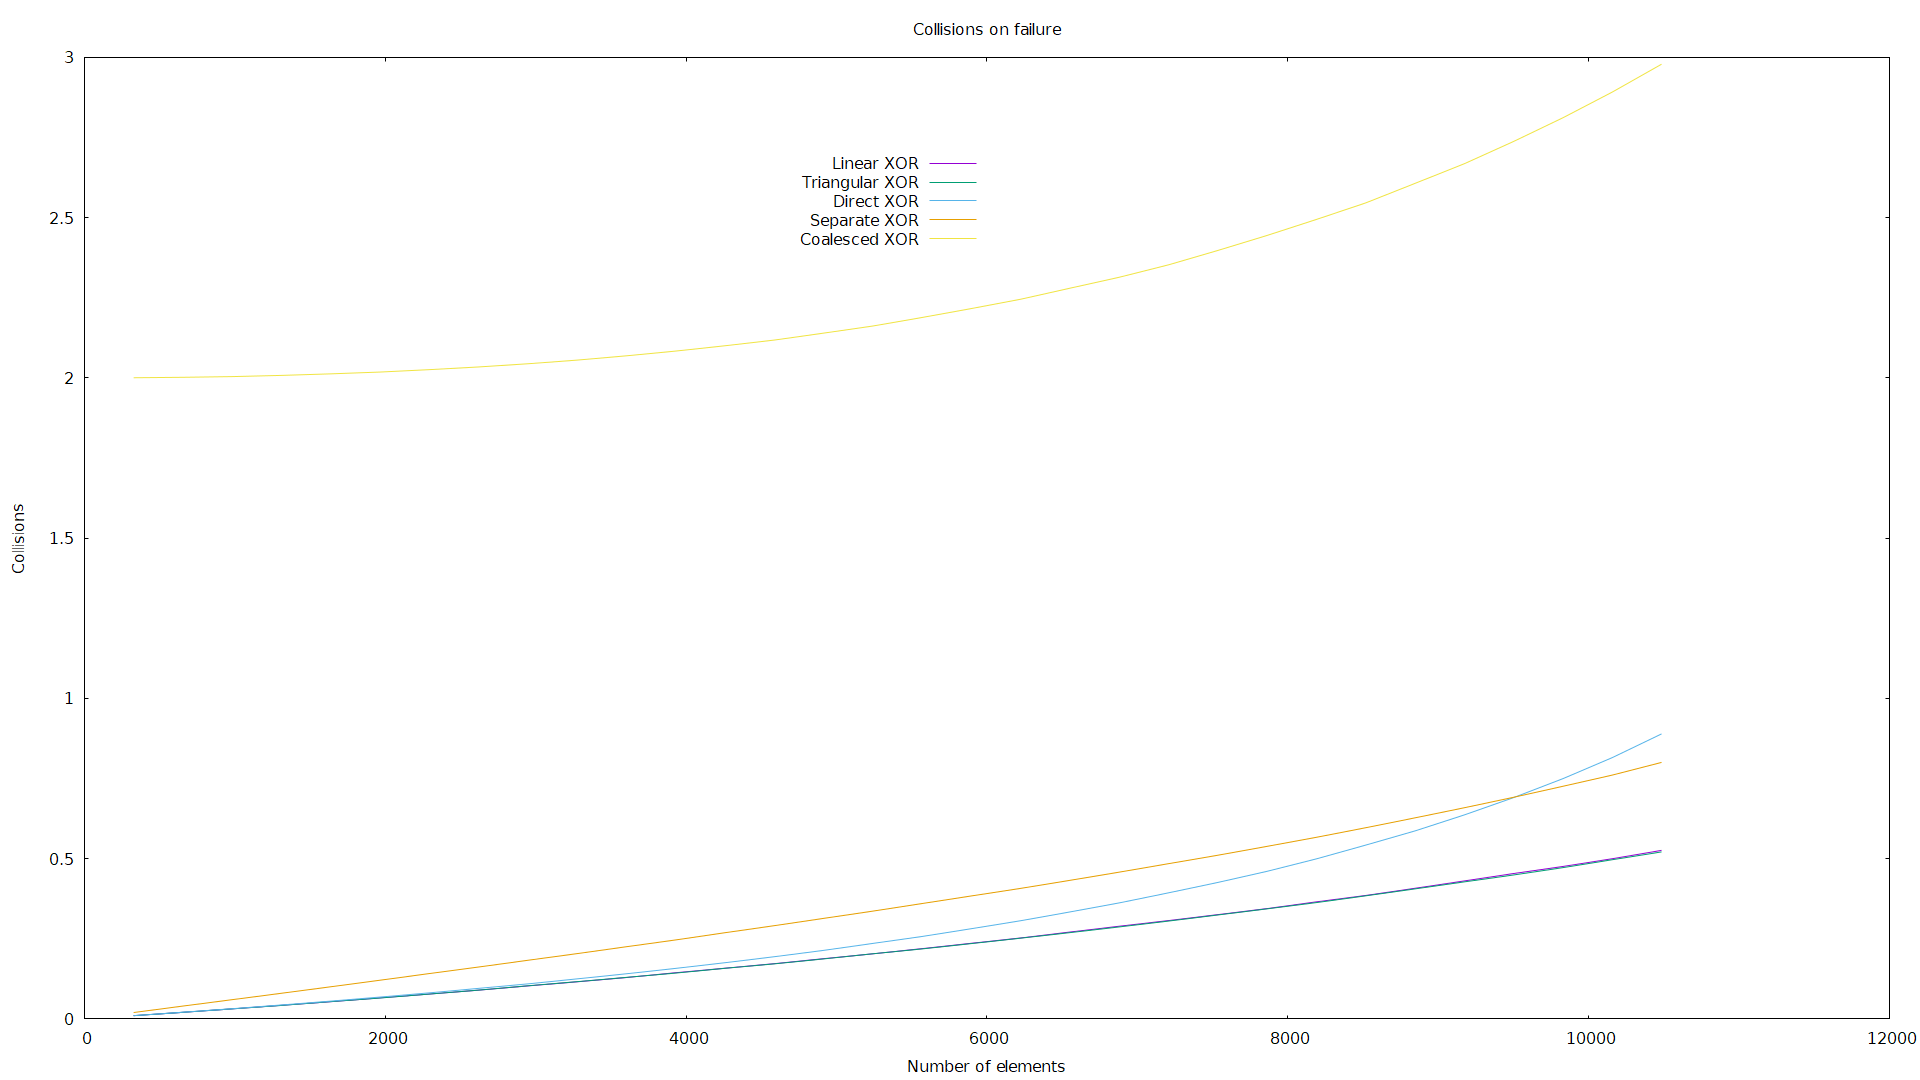
\includegraphics[width=0.7\paperwidth]{Bilder/failure_collisions_part.png}
    \caption{Durchschnittliche Anzahl an Kollisionen bei fehlschlagenden Zugriffen}
\end{figure}
\begin{figure}[h!]
    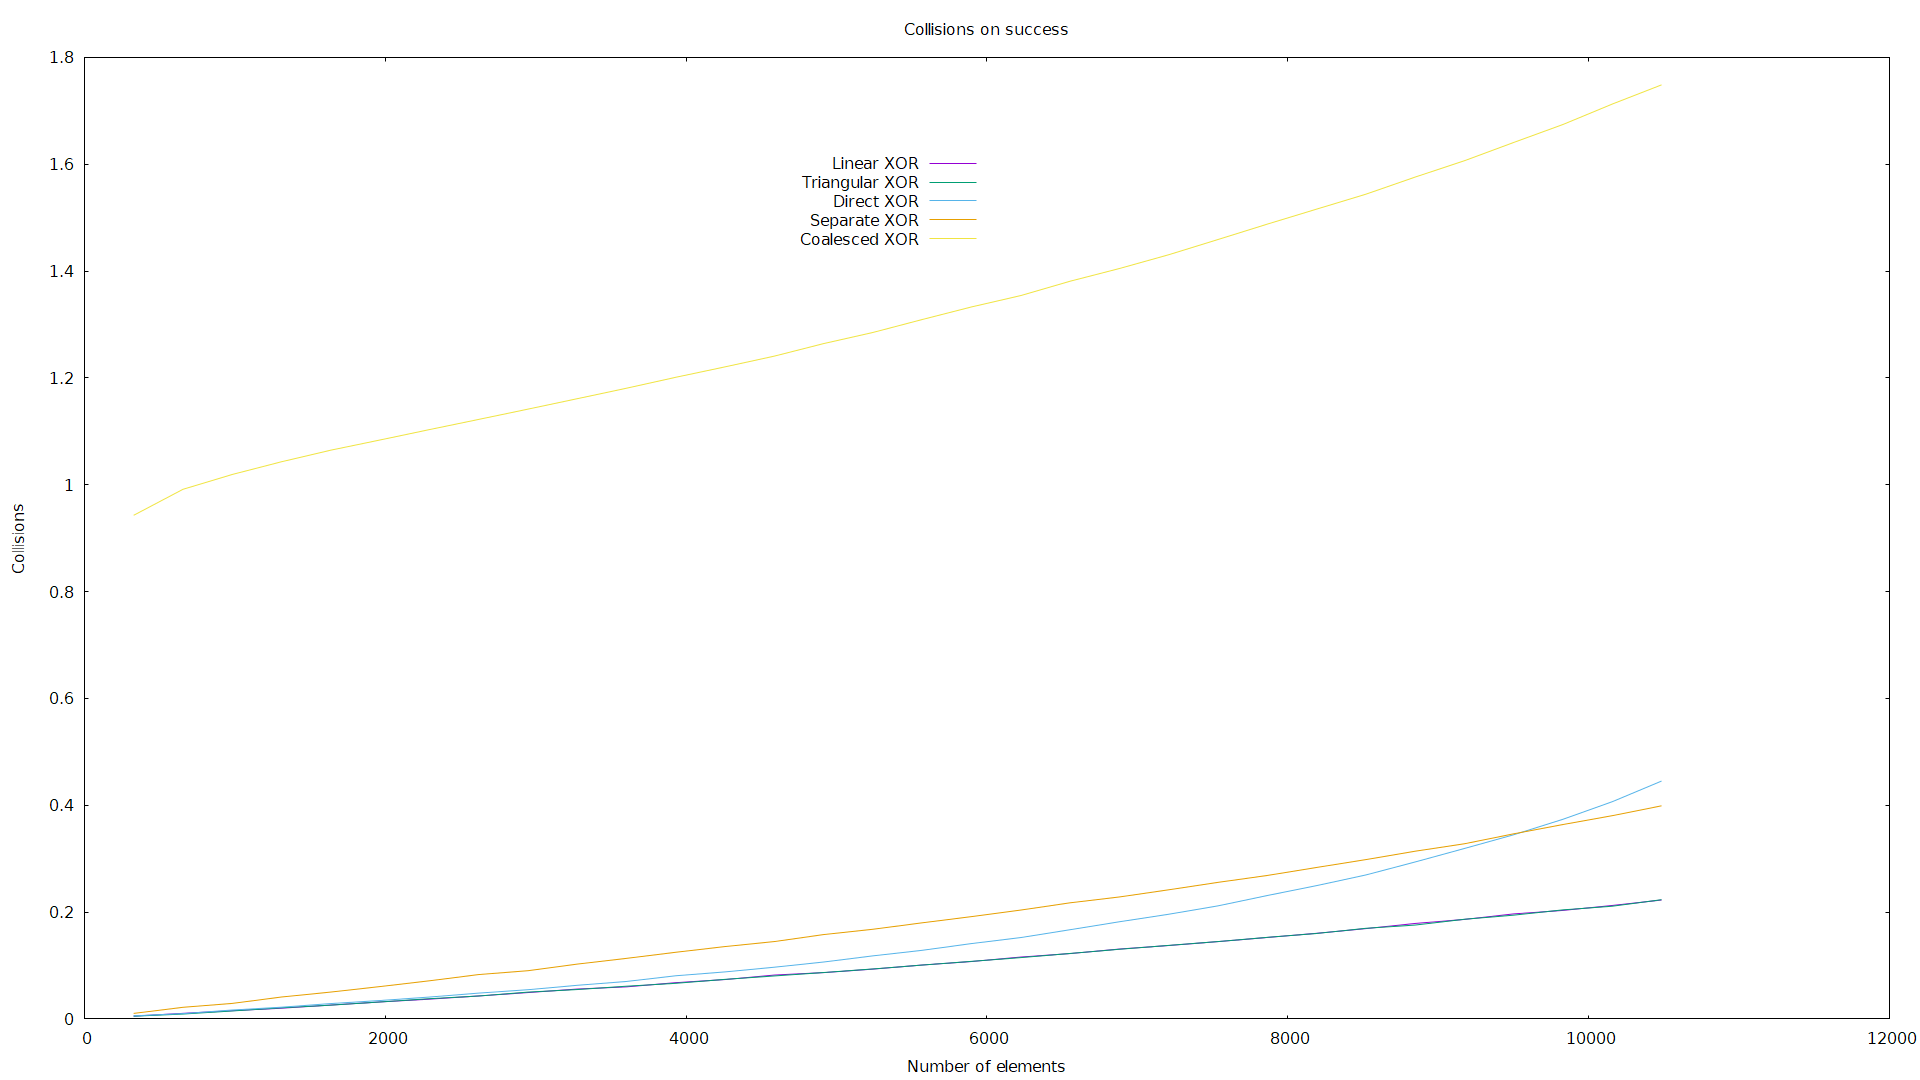
\includegraphics[width=0.7\paperwidth]{Bilder/successful_collisions_part.png}
    \caption{Durchschnittliche Anzahl an Kollisionen bei erfolgreichen Zugriffen}
\end{figure}
\begin{figure}[h!]
    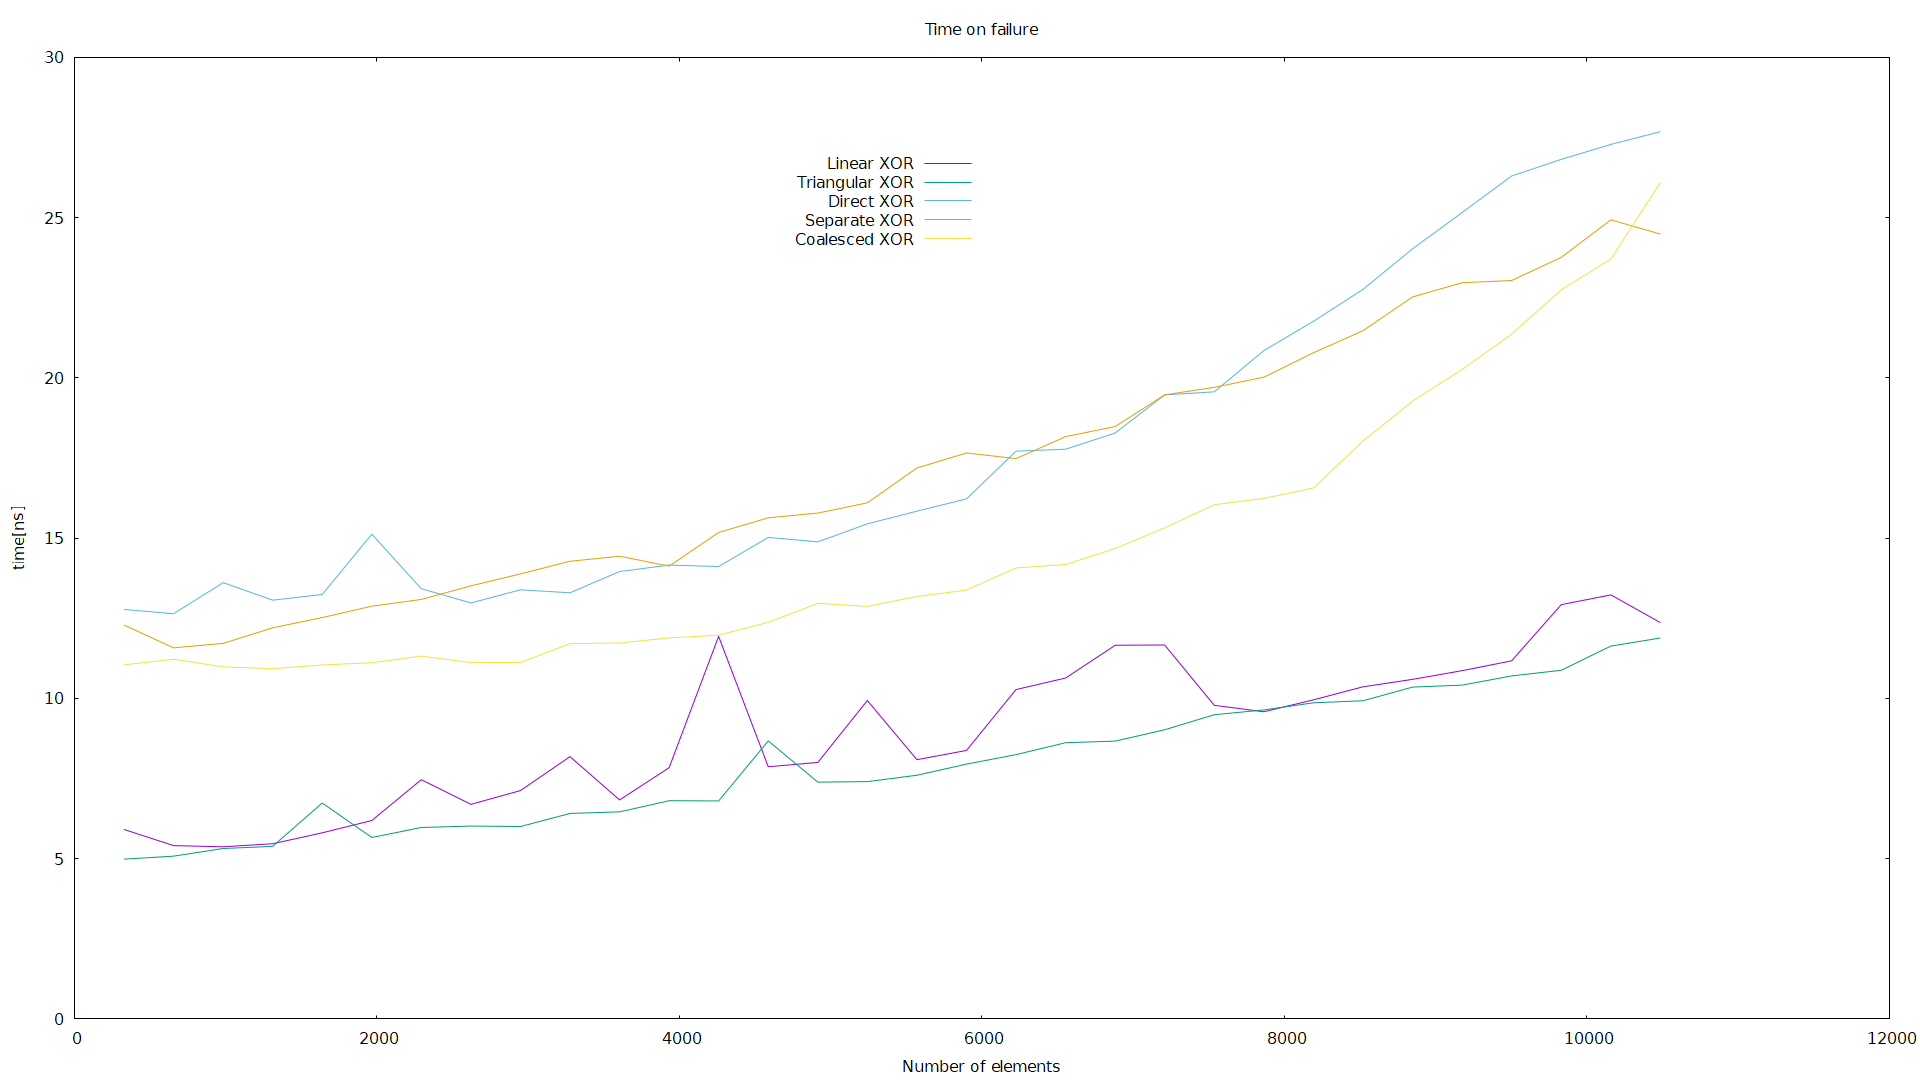
\includegraphics[width=0.7\paperwidth]{Bilder/failure_time_part.png}
    \caption{Durchschnittliche Zugriffszeit bei fehlschlagenden Zugriffen in ns}
\end{figure}
\begin{figure}[h!]
    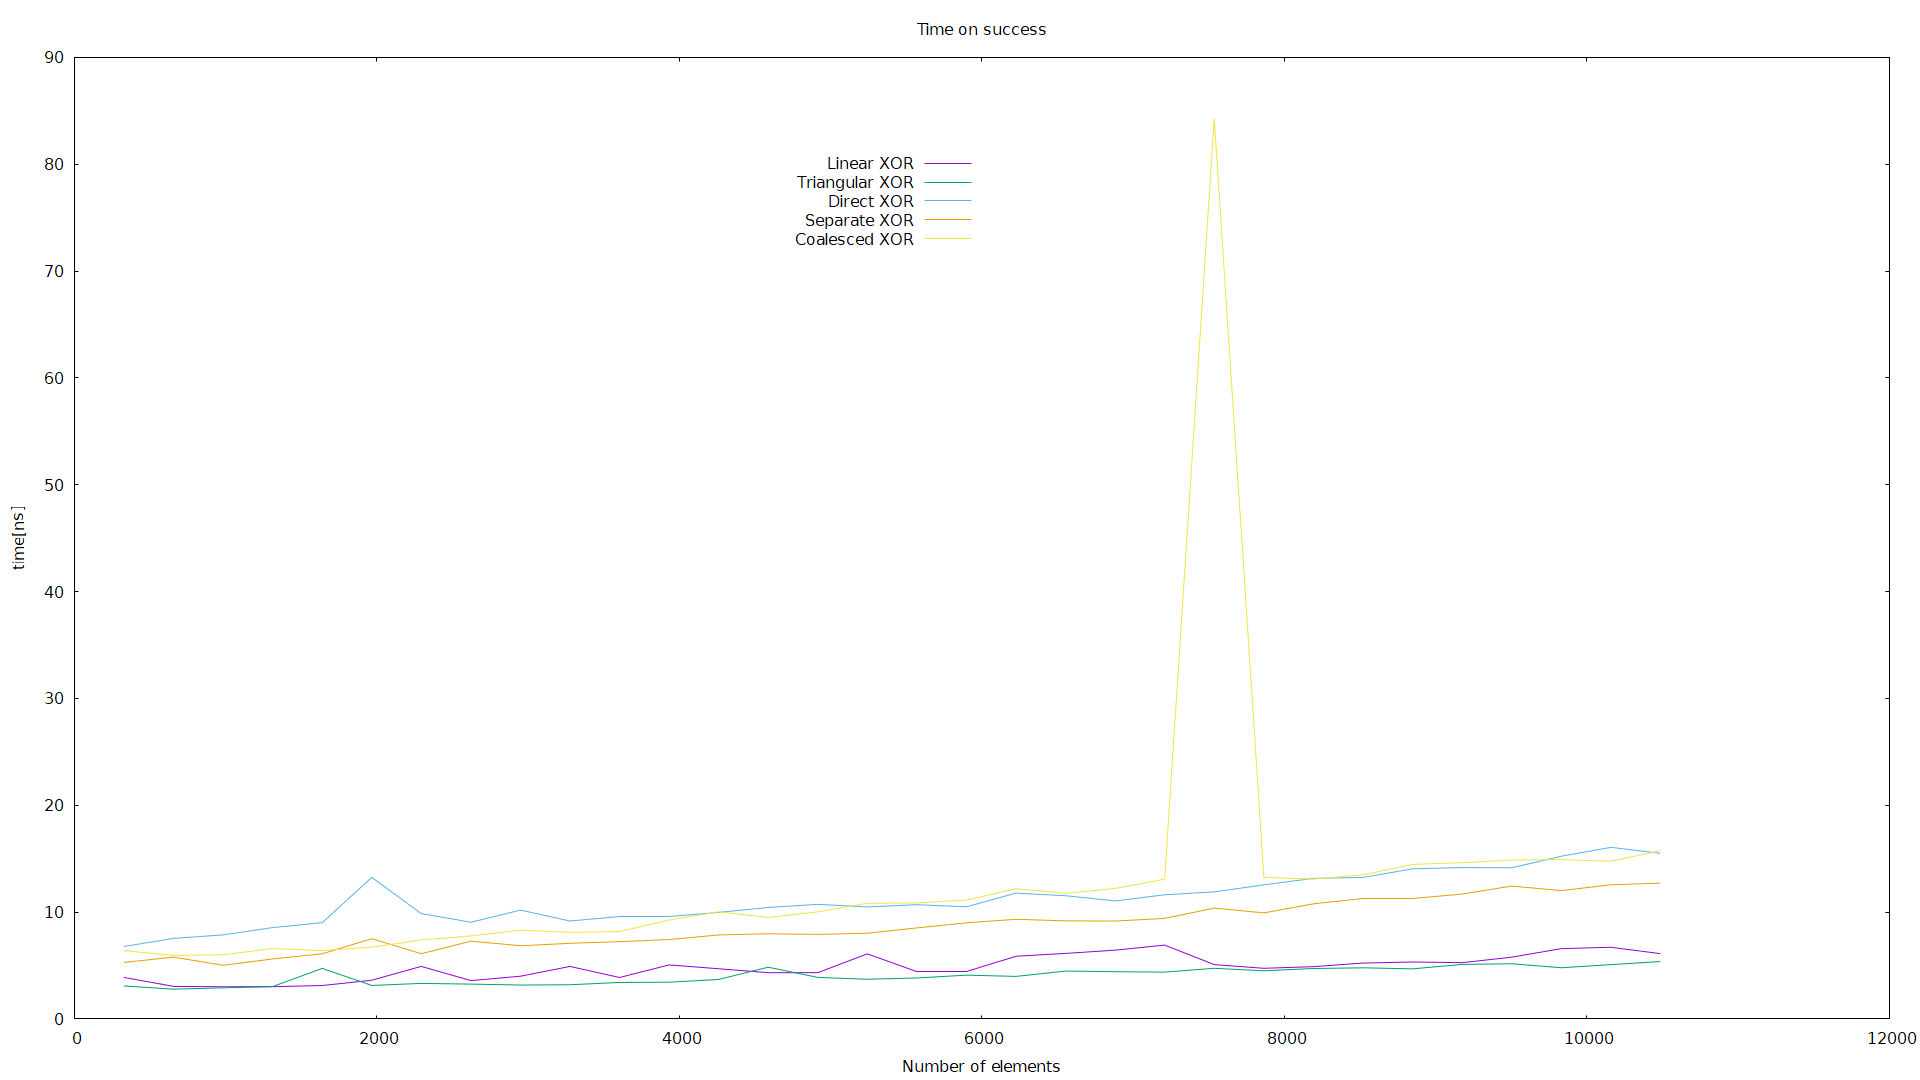
\includegraphics[width=0.7\paperwidth]{Bilder/successful_time_part.png}
    \caption{Durchschnittliche Zugriffszeit bei erfolgreichen Zugriffen in ns}
\end{figure}
\FloatBarrier